\documentclass{article}
\usepackage{tabularx,ragged2e,booktabs,caption}
\usepackage{graphicx}
\usepackage{float}
\usepackage{hyperref}
\usepackage{array}
\usepackage{graphicx}
\graphicspath{{imgs/}}
\usepackage{amsmath}
\usepackage{caption}
\usepackage{subcaption}
\usepackage{hyperref}
\usepackage{amssymb}

\newcommand{\kdtree}{\emph{k}-d tree}
\newcommand{\Mod}[1]{\ (\mathrm{mod}\ #1)}

\title{Implementation of a \kdtree{} using MPI and OpenMP}
\author{Francesco Andreuzzi}
\date{\today}

\begin{document}
\maketitle

\bibliographystyle{plain}

\section{Introduction}
A \kdtree{} is an established data structure which may be used to introduce
some structure in a dataset. Storing data in such a way enables the use of a
plethora of efficient algorithms such as \emph{nearest neighbor queries}
\cite{bentley1975multidimensional} which are of huge practical interest. Another
important aspect is the existence of efficient algorithms which enables updating
the data structure in response to changes in the dataset (deletion, insertion,
\dots).

In this brief report we present and analyze two parallel implementations of
\kdtree{} using two standard frameworks for parallel programming, namely OpenMP
\cite{dagum1998openmp} (shared memory) and MPI \cite{mpi} (distributed memory).
Our implementation uses quite the same approach for parallelization for both
cases, even though some compiler-level flags can be used to activate different
code regions which are more conceived in order to fix performance bottlenecks
which are peculiar of a particular framework (for instance \emph{false-sharing}
in OpenMP). We talk briefly about this point below.

First things first: we briefly discuss the data structure and the invariants to
be maintained. Afterwards we present the very simple parallel algorithm we
developed, and spend a few words on the implementation. We then procede with
some considerations on our expectations for the performance, and verify our
hypothesis against the real data we extracted from a set of run of the code.

\section{\kdtree{}}
Given a set of k-dimensional points $P = \{p^1, \dots, p^n\}$ such that
$p^i \in \mathbb{R}^k$ we pick a recursive definition of a \kdtree{}
\cite{skrodzki2019kd}: the node of the tree associated with the set $P$ is given
by:
\begin{gather} \label{eq:recursive_kdtree_definition}
    \text{Node}(P) = \begin{cases}
        \text{null} &\text{if } P = \emptyset\\
        \{p_m, \text{Node}(P_1), \text{Node}(P_2)\} &\text{otherwise}
    \end{cases}
\end{gather}
where $p_m$ is the median point of $P$ against some axis $i$ which is chosen
via an unspecified criteria which in some lines. $P_1, P_2 \subset P$ are
defined as follows:
\begin{gather*}
    P_1 = \{p \in P \mid p < p_m\} \qquad P_2 = \{p \in P \mid p > p_m\}
\end{gather*}
i.e. they are the subsets of points of $P$ which "fall" respectively before
and after $p_m$ along the i-th axis. For simplicity we assumed that $P$ does not
contain repeated values, however the definition is easily generalized.
$\text{Node}(P_1), \text{Node}(P_2)$ in (\ref*{eq:recursive_kdtree_definition})
are respectively the left and right branch which originate from
$\text{Node}(P)$.

The axis $i$ is chosen in such a way that the spread of the points in $P$ is
maximum along $i$. However, since we assumed that our points are distributed
somewhat uniformly in the space $\mathbb{R}^k$, we are going to use a very
simple function to determine the axis $i$ used to "split" the tree:
\begin{gather*}
    i(\ell) = \ell \Mod{k}
\end{gather*}
where $\ell$ is the current level of the tree (i.e. the distance of the current
node from the root).

Using a
\href{https://github.com/fAndreuzzi/parallel-kd-tree/tree/master/visualization}{visualizer tool}
written in Python which we developed for the occasion, we show the progression
of the construction of a \kdtree{} for a very simple dataset.

\begin{figure}[b!]
    \makebox[\textwidth][c]{
        \begin{subfigure}{.4\textwidth}
            \centering
            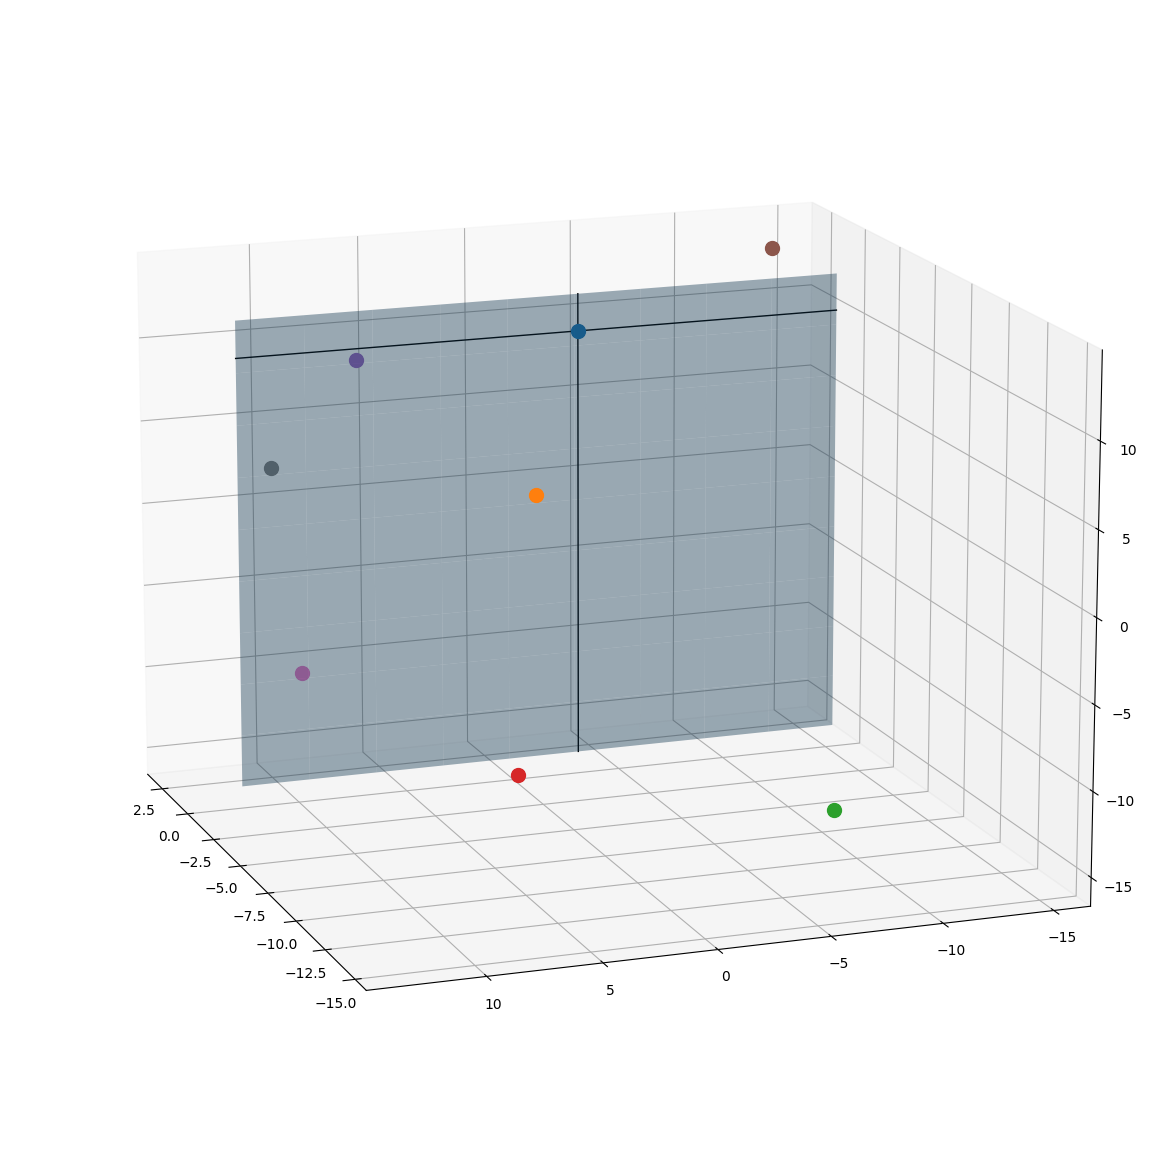
\includegraphics[width=\linewidth]{kd_tree_progress_img0.png}
            \caption{Depth 0}
        \end{subfigure}%
        \hfill
        \begin{subfigure}{.4\textwidth}
            \centering
            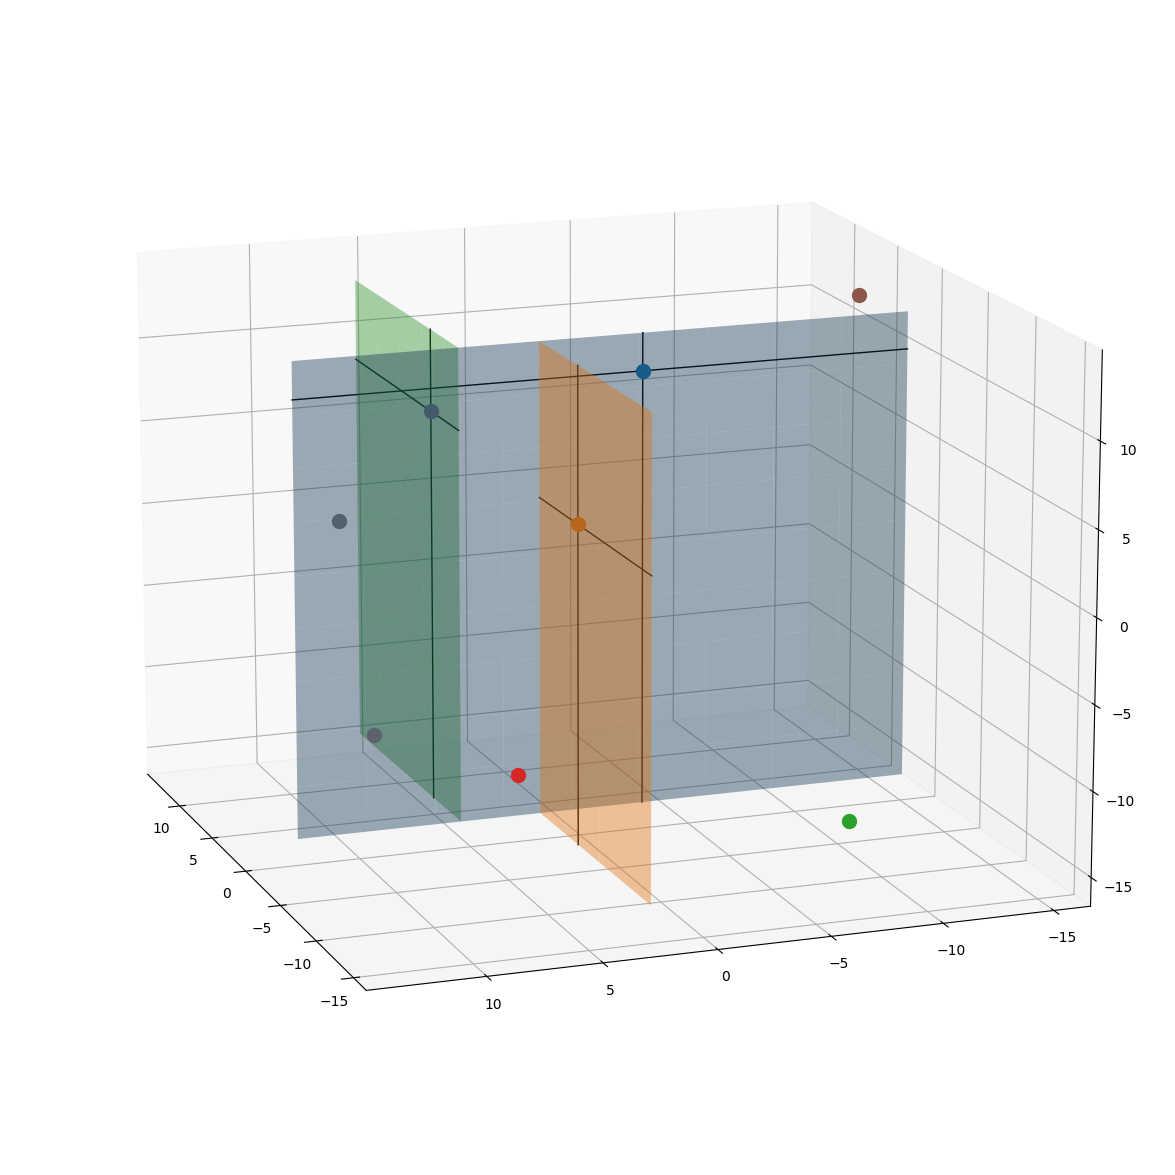
\includegraphics[width=\linewidth]{kd_tree_progress_img1.png}
            \caption{Depth 1}
        \end{subfigure}
        \hfill
        \begin{subfigure}{.4\textwidth}
            \centering
            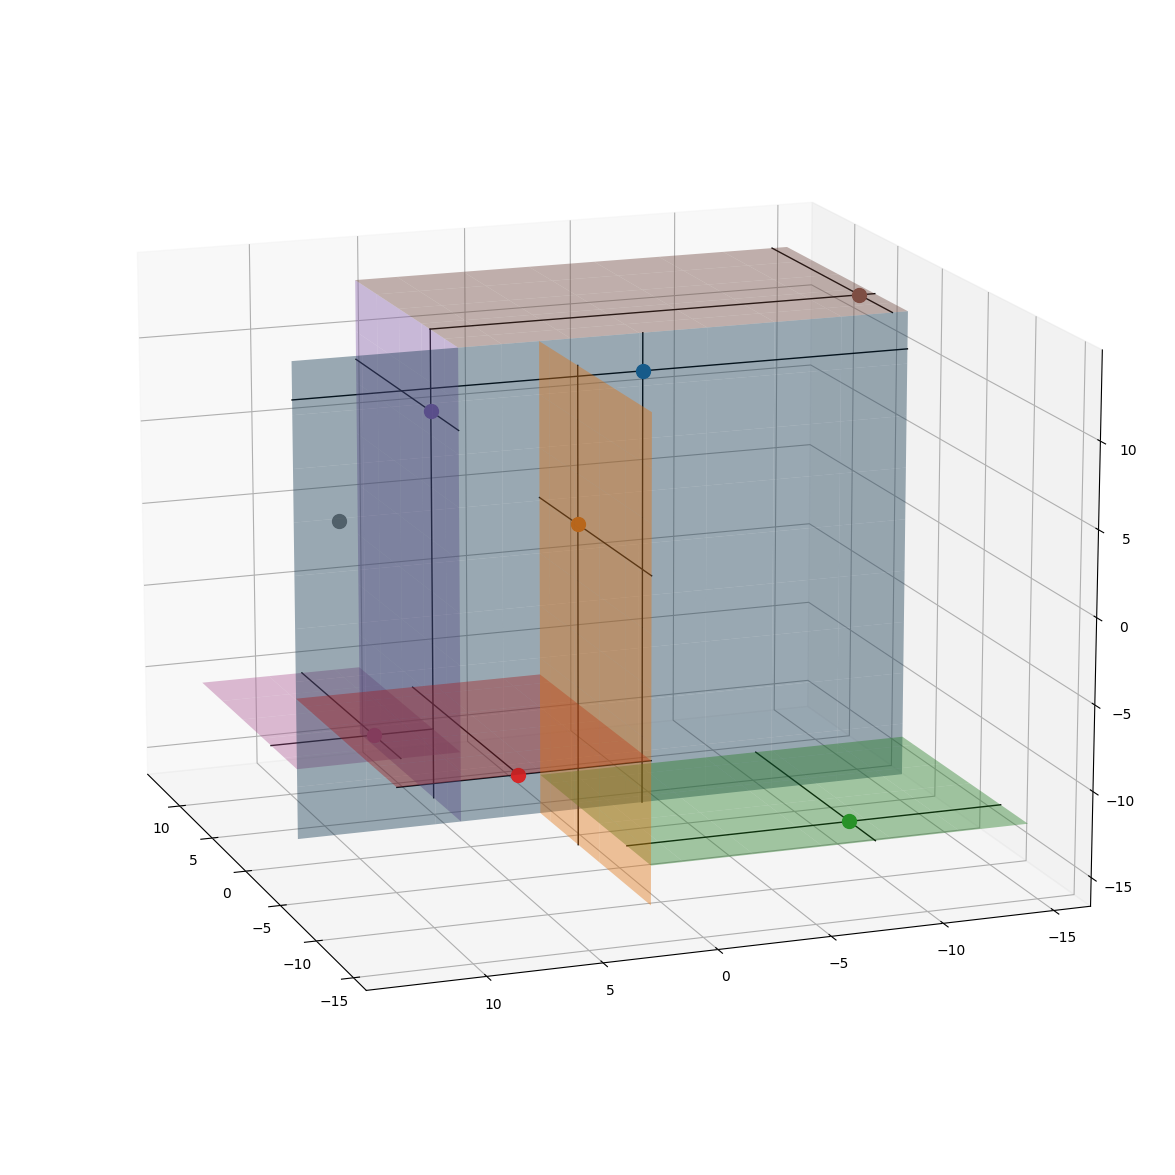
\includegraphics[width=\linewidth]{kd_tree_progress_img2.png}
            \caption{Depth 2}
        \end{subfigure}
    }
    \caption{A \kdtree{} (surfaces representation).}
    \label{fig:kdtree_surfaces_progression}
\end{figure}

The visualization in Figure \ref{fig:kdtree_surfaces_progression} renders in a
very clear way the fact that points added to the tree in the level $k$ need to
satisfy constraints given by all the points in the parent branches in levels
$0, \dots, k-1$. Each surface is the plane containing one of the points
added to the tree in the current level, which divides the volume dedicated to
the corresponding branch in two halves which shall contain all the other points
(respectively) in the left and right branch. This is almost a visual
transposition of (\ref*{eq:recursive_kdtree_definition}).

However, in order to communicate the structure of the tree
the visualization shown in Figure \ref{fig:kdtree_branches_progression} may be
preferred, which is easier to interpret visually but conveys a smaller amount
of information about the structure we imposed on the dataset.

\begin{figure}[t!]
    \makebox[\textwidth][c]{
        \begin{subfigure}{.4\textwidth}
            \centering
            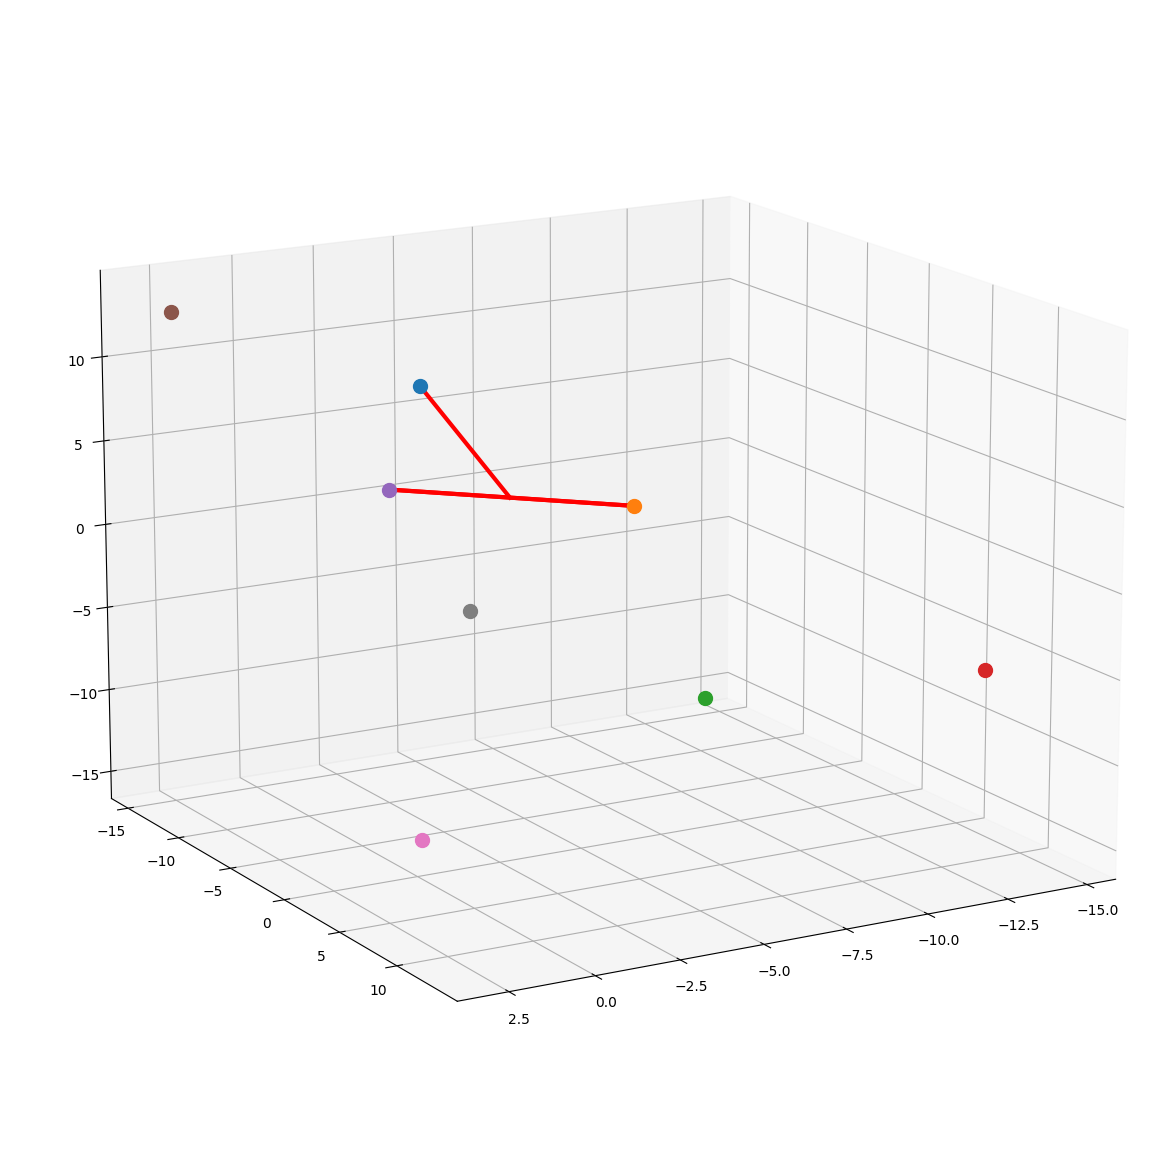
\includegraphics[width=\linewidth]{kd_tree_progress_img0_branches.png}
            \caption{Depth 0}
            \end{subfigure}%
        \hfill
        \begin{subfigure}{.4\textwidth}
            \centering
            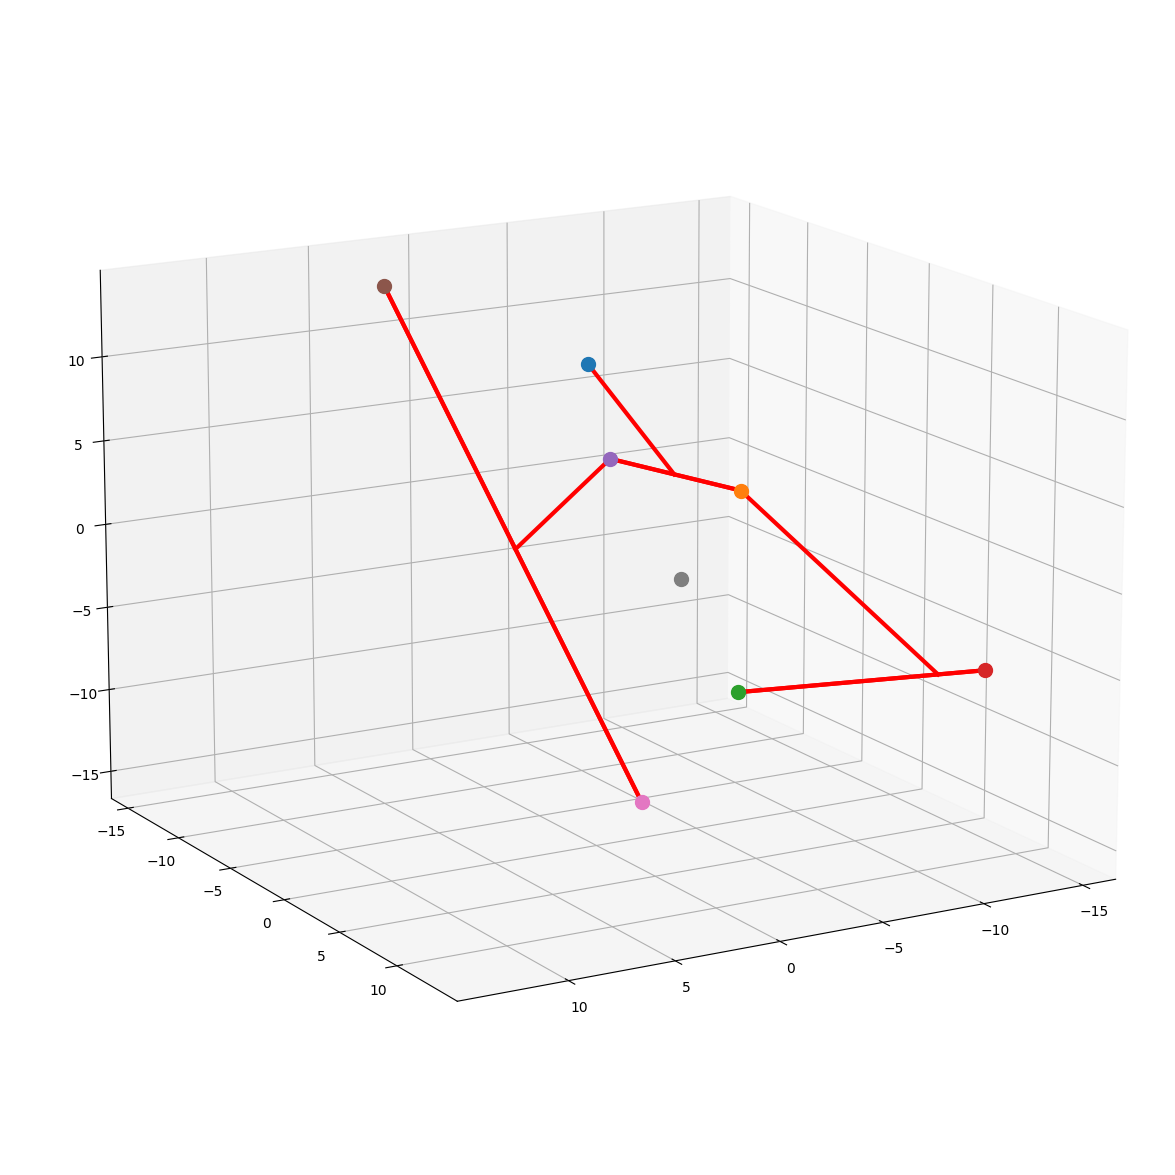
\includegraphics[width=\linewidth]{kd_tree_progress_img1_branches.png}
            \caption{Depth 1}
            \end{subfigure}
        \hfill
        \begin{subfigure}{.4\textwidth}
            \centering
            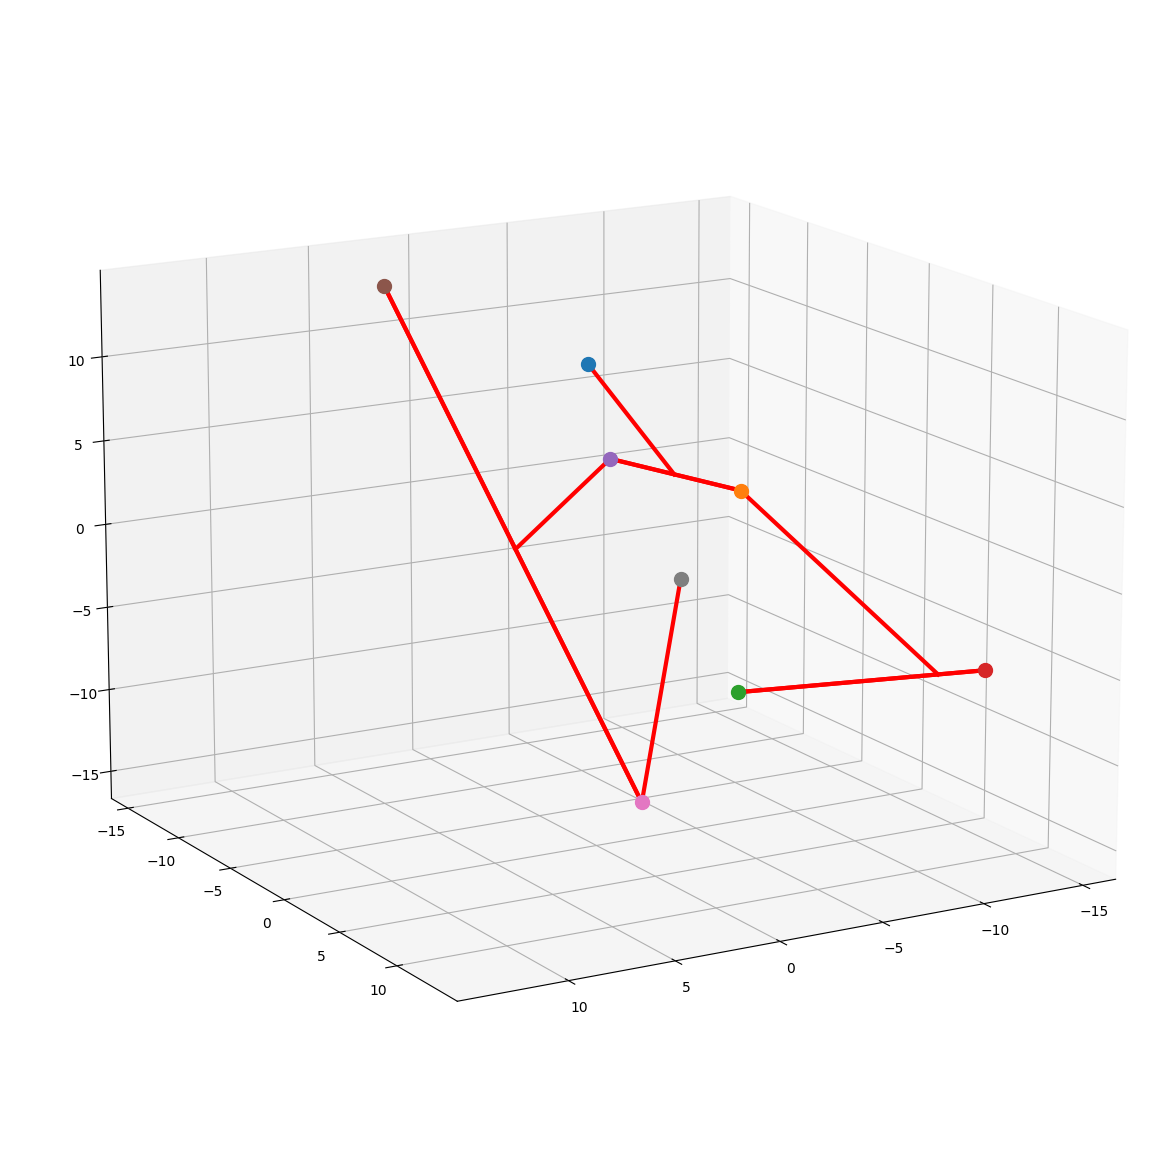
\includegraphics[width=\linewidth]{kd_tree_progress_img2_branches.png}
            \caption{Depth 2}
        \end{subfigure}
    }
    \caption{The same \kdtree{} shown in Figure \ref{fig:kdtree_surfaces_progression} (branches representation).}
    \label{fig:kdtree_branches_progression}
\end{figure}

\section{Algorithm and implementation}

\section{Performance model and results}

\section{Conclusions}

\bibliography{bibfile}

\end{document}
